\subsection{Alternating bit protocol - modelling, specification and verification}

The alternating bit protocol is a simple yet effective protocol (usually used as a test case), designed to ensure reliable communication through unreliable transmission mediums, and it is used for managing the retransmission of lost messages \cite{ReactiveSystems}\cite{Kulick}.

\subsubsection{Modelling and Specification.}
The representation of the Alternating Bit Protocol consists of a $sender$ $S$, a $receiver$ $R$ and two channels $transport$ $T$ and $acknowledge$ $A$ as shown below. 

\begin{figure}[h]
\centering
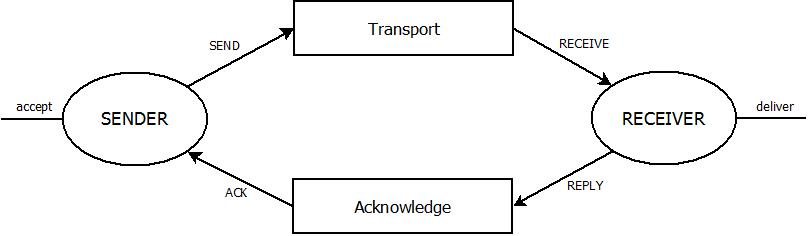
\includegraphics[width=4.5in]{abp}
\caption{Alternating Bit Protocol representation}
\label{fig:abp}
\end{figure}

The only visible transitions in the alternating bit protocol are $deliver$ and $accept$, which can occur only sequentially, whereas all others are internal synchronizations. Sender $S$ sends a message which contains the protocol bit, 0 or 1, to a receiver $R$. The channel from $S$ to $R$ is initialized and there are no messages in transit. There is no direct communication between the sender $S$ and the receiver $R$, and all messages must travel trough the medium ($transport$ and $acknowledge$ channel). 

The functioning of the alternating bit protocol can be described as follows \cite{ReactiveSystems}:
\begin{enumerate}
	\item The sender $S$ sends a message repeatedly (with its corresponding bit) until it receives an acknowledgment ($ack0$ or $ack1$) from the receiver $R$ that contains the same protocol bit as the message being sent. This behaviour of the process representing the sender can be described as:
				\begin{equation*}\label{send_imp}
				    \begin{array}{lcl}
							S = \overline{send0}.S+ack0.accept.S_{1}+ack1.S \\
							S_{1}=\overline{send1}.S_{1}+ack1.accept.S+ack0.S_{1}				  
						\end{array}
				\end{equation*}
	      The transport channel transmits the message to the receiver, but it may lose the message (lossy channel) or transmit it several times (chatty channel). Therefore, the description of the behaviour of the process representing the transport channel is given with CCS expression as follows:
	      \begin{equation*}\label{trans_imp}
	      	\begin{array}{lcl}
						T=send0.\left(T+T_{1}\right)+send1.\left(T+T_{2}\right)\\
						T_{1}=\overline{receive0}.\left(T+T_{1}\right)\\
						T_{2}=\overline{receive1}.\left(T+T_{2}\right)
					\end{array}
				\end{equation*}
  \item When the receiver $R$ receives a message, it sends a reply to $S$ which includes the protocol bit of the message received. When the message is received for the first time, the receiver will deliver it for processing, while subsequent messages with the same bit will be simply acknowledged. That yields the following CCS expression for the receiver:
  			\begin{equation*}\label{rec_imp}
				    \begin{array}{lcl}
							R=receive0.\overline{deliver}.R_{1}+\overline{reply1}.R+receive1.R \\
							R_{1}=receive1.\overline{deliver}.R+\overline{reply0}.R_{1}+receive0.R_{1}			  
						\end{array}
				\end{equation*}
        Again, the acknowledgement channel sends the $ack$ to sender, and it can also acknowledge it several times or lose it on the way to the sender. Therefore the CCS expression describing the ackowledgement channel and its behaviour is given as follows:
        \begin{equation*}\label{trans_imp}
	      	\begin{array}{lcl}
						A=reply0.\left(A+A_{1}\right)+reply1.\left(A+A_{2}\right)\\
						A_{1}=\overline{ack0}.\left(A+A_{1}\right)\\
						A_{2}=\overline{ack1}.\left(A+A_{2}\right)
					\end{array}
				\end{equation*}
  \item When $S$ receives an acknowledgment containing the same bit as the message it is currently transmitting, it stops transmitting that message, flips the protocol bit, and repeats the protocol for the next message.\cite{Kulick}\cite{ProcessAlgebraParallel}
\end{enumerate}

Having described the behaviour of the alternating bit protocol components, the CCS process expression describing the behaviour of the protocol as a whole can be obtained as a parallel composition of the processes describing the sender, the transport channel, the receiver and the acknowledgement channel:
\begin{equation}\label{abp_imp}
	\mathit{ABP} \stackrel{def}{=}\left(S|T|R|A\right)\backslash L,
\end{equation}
restricted on the set of actions:
\begin{equation*}
  L = \left(send0,send1,receive0,receive1,reply0,reply1,ack0,ack1\right)
\end{equation*}

This CCS expression represents the implementation of the alternating bit protocol which details the proposed means for achieving the desired high-level behaviour the alternating bit protocol should exhibit. This desired high-level behaviour is that the alternating bit protocol should act as a simple buffer, therefore its CCS specification is defined as follows:
\begin{equation}\label{eq:abp_spec}
	\begin{array}{lcl}
		\mathit{Buf} = \mathit{accept.Buf'}\\
		\mathit{Buf'} = \mathit{\overline{deliver}.Buf}
	\end{array}
\end{equation}

\subsubsection{Verification.} In order to verify the alternating bit protocol, we need to prove that the implementation $ABP$ meets the specification $Buf$ with respect to some behavioural equivalence. We shall show that an observational equivalence between $\mathit{Buf}$ and $\mathit{ABP}$ can be found, i.e. that $\mathit{ABP}\approx \mathit{Imp}$. For that purpose, first we use TMACS to obtain the labeled graphs corresponding to the CCS representations of $\mathit{Buf}$ and $\mathit{ABP}$, and afterwards we perform a comparison of the labeled transition systems modulo weak bisimilarity which yields a positive answer about the existance of weak bisimulation equivalence between $\mathit{Buf}$ and $\mathit{ABP}$.

The weak bisimulation equivalence obtained by running any of the two bisimulation algorithms implemented in TMACS over the saturated labeled transition systems is given in Table~\ref{table3}:

\begin{table}
\begin{tabular}{| p{6.5cm} | p{3.5cm} | }
	
  \hline                       
	ABP implementation states &
	ABP specification states
	\\ \hline
	
$\left(S|T|R|A\right)\backslash L$ & \\
$\left(S|\left(T+T1\right)|R|A\right)\backslash L$ & \\
$\left(S|\left(T+T1\right)|R|\left(A+A2\right)\right)\backslash L$ & \\
$\left(S|T|R|\left(A+A2\right)\right)\backslash L$ & \\
$\left(S|\left(T+T1\right)|\overline{deliver}.R1|A\right)\backslash L$ & \\
$\left(S|\left(T+T1\right)|\overline{deliver}.R1|\left(A+A2\right)\right)\backslash L$ & \\
$\left(S1|\left(T+T1\right)|R1|\left(A+A1\right)\right)\backslash L$ & \\
$\left(S1|\left(T+T2\right)|\overline{deliver}.R|\left(A+A1\right)\right)\backslash L$ & \\
$\left(S1|\left(T+T2\right)|R1|\left(A+A1\right)\right)\backslash L$ & \\
$\left(S|\left(T+T2\right)|R|\left(A+A2\right)\right)\backslash L$ &
  $\mathit{Buf}$   
  \\ \hline
   
$\left(accept.S1|\left(T+T1\right)|R1|\left(A+A1\right)\right)\backslash L$ & \\ 
$\left(S|\left(T+T1\right)|R1|\left(A+A1\right)\right)\backslash L$ & \\
$\left(S|\left(T+T1\right)|R1|\left(A+A2\right)\right)\backslash L$ & \\
$\left(S|\left(T+T1\right)|R1|A\right)\backslash L$ & \\
$\left(S1|\left(T+T2\right)|R|\left(A+A2\right)\right)\backslash L$ & \\
$\left(accept.S|\left(T+T2\right)|R|\left(A+A2\right)\right)\backslash L$ & \\
$\left(S1|\left(T+T2\right)|R|\left(A+A1\right)\right)\backslash L$ &
  $\mathit{Buf'}$
  \\ \hline  
\end{tabular}
\\
\caption{Verification of the alternating bit protocol using weak bisimilarity}
\label{table3}
\end{table}
